\documentclass[aspectratio=169, 11pt]{beamer}

\usepackage[T2A]{fontenc}
\usepackage[utf8]{inputenc}
\usepackage[russian]{babel}
\usepackage{amsmath}
\usepackage{graphicx}
\usepackage{booktabs}
\usepackage{array}
\usepackage{hyperref}

\usetheme{Boadilla}
\usecolortheme{default}
\setbeamertemplate{navigation symbols}{}
\setbeamertemplate{footline}[frame number]

\graphicspath{{../../code/paper_figures/}}

\title[Флуктуации поверхностной яркости]{Улучшение точности измерения расстояний в ближней Вселенной по флуктуациям поверхностной яркости галактик}
\author{\texorpdfstring{Буканов И.\,А. }{Буканов И.А. }}
\institute{ФКИ МГУ\\[0.25cm]\small Научный руководитель: к.ф.-м.н. Афанасьев А.\,А., ГАИШ МГУ}
\date{2026}

\begin{document}

\begin{frame}
    \titlepage
\end{frame}

\begin{frame}{Задача работы}
    \begin{block}{Цель}
        Построить рабочий пайплайн измерения SBF по данным JWST/NIRCam F150W и получить эмпирическую калибровку расстояний.
    \end{block}
    \vspace{0.2cm}
    \begin{itemize}
        \item измерить $\bar{m}_{150}$ для галактик программы JWST GO-3055;
        \item оценить бюджет ошибок по схеме, близкой к Jensen et al.;
        \item откалибровать $\bar{M}_{150}$ через цвет $F090W-F150W$;
        \item проверить расстояния относительно TRGB и HST/F160W SBF.
    \end{itemize}
\end{frame}

\begin{frame}{Идея метода SBF}
    \begin{columns}[T]
        \begin{column}{0.53\textwidth}
            \begin{itemize}
                \item Неразрешённая галактика не является идеально гладкой.
                \item Число ярких звёзд в пикселях флуктуирует.
                \item После вычитания гладкой модели остаётся статистический сигнал.
                \item Чем дальше галактика, тем слабее видимые флуктуации.
            \end{itemize}
        \end{column}
        \begin{column}{0.43\textwidth}
            \begin{equation*}
                \bar{m} = \bar{M} + \mu
            \end{equation*}
            \begin{equation*}
                \mu = \bar{m}_{150} - \bar{M}_{150}(C)
            \end{equation*}
            \begin{equation*}
                C = F090W-F150W
            \end{equation*}
        \end{column}
    \end{columns}
    \vspace{0.25cm}
    \begin{block}{Ключевая точка}
        Мы измеряем видимую SBF-величину $\bar{m}_{150}$, а затем калибруем абсолютную величину $\bar{M}_{150}$ по независимой TRGB-шкале.
    \end{block}
\end{frame}

\begin{frame}{Данные}
    \begin{itemize}
        \item JWST/NIRCam, программа GO-3055, публичные i2d-продукты MAST.
        \item Основной фильтр: F150W, в нём измеряется $\bar{m}_{150}$.
        \item Цвет: $F090W-F150W$ в тех же областях галактики.
        \item Обработано 14 галактик; основная калибровочная выборка: 12 объектов.
        \item Литературные расстояния: TRGB-SBF Project IV.
        \item Внешнее SBF-сравнение: Jensen et al. 2015, HST/WFC3 F160W.
    \end{itemize}
    \vspace{0.15cm}
    \begin{block}{Почему не Cepheid/SN Ia прямо в калибровке}
        Объекты выборки -- в основном ранние галактики. Для них нет однородной прямой шкалы Cepheid/SN Ia, поэтому такая калибровка добавила бы неоднородную систематику. TRGB используется как единая независимая опорная шкала.
    \end{block}
\end{frame}

\begin{frame}{Какие шкалы сравниваются}
    \scriptsize
    \setlength{\tabcolsep}{3pt}
    \begin{tabular}{>{\raggedright\arraybackslash}p{0.21\textwidth}
                    >{\raggedright\arraybackslash}p{0.29\textwidth}
                    >{\raggedright\arraybackslash}p{0.42\textwidth}}
    \toprule
    Источник & Что берём & Зачем нужен в работе \\
    \midrule
    Эта работа & $\mu_{150}$ из JWST/NIRCam F150W SBF & Основной результат: расстояния после новой цветовой калибровки $\bar{M}_{150}(F090W-F150W)$. \\
    TRGB-SBF Project IV & $\mu_{\rm TRGB}$ для всех 14 галактик & Опорная независимая шкала для нуль-пункта и проверки среднего смещения. \\
    Jensen et al. 2015 & HST/WFC3 F160W SBF для 5 общих галактик & Внешняя проверка против другой реализации SBF-метода и другой фотометрической шкалы. \\
    \bottomrule
    \end{tabular}

    \vspace{0.25cm}
    \begin{block}{Принцип}
        На графиках показываются не конкурирующие fit-ы, а сравнение шкал расстояний.
        TRGB задаёт опору нуль-пункта; Jensen/F160W проверяет согласие с опубликованной IR SBF-шкалой.
    \end{block}
\end{frame}

\begin{frame}{Пайплайн обработки}
    \begin{enumerate}
        \item вычитание фона и построение маски компактных источников;
        \item построение гладкой изофотной модели галактики;
        \item получение остаточного изображения;
        \item измерение спектра мощности $P(k)$ в кольцевых областях;
        \item подгонка $P(k)=P_0E(k)+P_1$;
        \item поправка за неразрешённые источники: $P_{\rm fluc}=P_0-P_r$;
        \item перевод $P_{\rm fluc}$ в $\bar{m}_{150}$.
    \end{enumerate}
    \vspace{0.15cm}
    \begin{block}{Контроль качества}
        Остатки и маски проверялись визуально; реальные проблемные флаги оставлены для NGC 4621 и NGC 4697.
    \end{block}
\end{frame}

\begin{frame}{Как строилась модель галактики}
    \begin{itemize}
        \item Сначала строилась первичная модель Серсика: она нужна для заполнения NaN и центральной области, а не как финальная SBF-модель.
        \item Основная гладкая модель строилась по эллиптическим изофотам с плавающим центром, эллиптичностью и позиционным углом.
        \item Изофоты считались настолько далеко, насколько они устойчиво сходились; дальше модель не принудительно обрезалась.
        \item Это важно: граница между ``изофотной'' и ``достроенной'' частью не должна проявляться в остатках.
    \end{itemize}
    \begin{block}{Что контролировалось глазами}
        Проверялись модель, остаток image--model и финальный residual в SBF-области. Явные скачки модели или недовычитанные крупномасштабные структуры считались проблемой пайплайна.
    \end{block}
\end{frame}

\begin{frame}{Как получался остаток для SBF}
    \begin{enumerate}
        \item из F150W-кадра вычиталась гладкая модель галактики;
        \item компактные источники маскировались до и после построения остатка;
        \item дополнительно вырезались положительные компактные residual-объекты: шаровые скопления, фоновые галактики, звёзды;
        \item измерение SBF велось в двух фиксированных кольцах: $8.2$--$16.4''$ и $16.4$--$32.8''$.
    \end{enumerate}
    \vspace{0.15cm}
    \begin{block}{Почему это не ``подгонка картинки под ответ''}
        Маска убирает компактные источники, но не SBF-сигнал: SBF -- пространственно распределённая статистическая мощность, а не отдельные яркие пятна.
    \end{block}
\end{frame}

\begin{frame}{Как фиттился спектр мощности $P(k)$}
    \begin{columns}[T]
        \begin{column}{0.50\textwidth}
            \begin{equation*}
                P(k)=P_0E(k)+P_1
            \end{equation*}
            \begin{itemize}
                \item $P(k)$ -- спектр мощности остаточного изображения;
                \item $E(k)$ -- ожидаемая форма SBF-сигнала: PSF, свёрнутая с маской;
                \item $P_0$ -- амплитуда SBF;
                \item $P_1$ -- белый шум;
                \item рабочее окно: $k=0.01$--$0.25$ cycles/pixel.
            \end{itemize}
        \end{column}
        \begin{column}{0.46\textwidth}
            \begin{block}{Почему низкие и высокие частоты ограничены}
                Слишком малые $k$ чувствительны к остаткам модели галактики, слишком большие $k$ -- к пиксельному шуму и деталям PSF. Окно выбрано после диагностики формы $P(k)$.
            \end{block}
            \begin{equation*}
                P_{\rm fluc}=P_0-P_r
            \end{equation*}
        \end{column}
    \end{columns}
\end{frame}

\begin{frame}{Бюджет ошибок $\bar{m}_{150}$}
    \begin{columns}[T]
        \begin{column}{0.52\textwidth}
            \begin{equation*}
                \sigma_{\bar{m}}^2 =
                \sigma_{P(k)}^2 + \sigma_{\rm bkg}^2 +
                \sigma_{\rm PSF}^2 + \sigma_{P_r}^2 + \sigma_{\rm ext}^2
            \end{equation*}
            \begin{itemize}
                \item главный вклад обычно даёт $\sigma_{P(k)}$;
                \item PSF меньше по величине, но важен систематически;
                \item $P_r$ учитывает слабые шаровые скопления и фоновые галактики;
                \item $\sigma_{\rm int}$ не входит сюда: это ширина калибровки расстояний.
            \end{itemize}
        \end{column}
        \begin{column}{0.45\textwidth}
            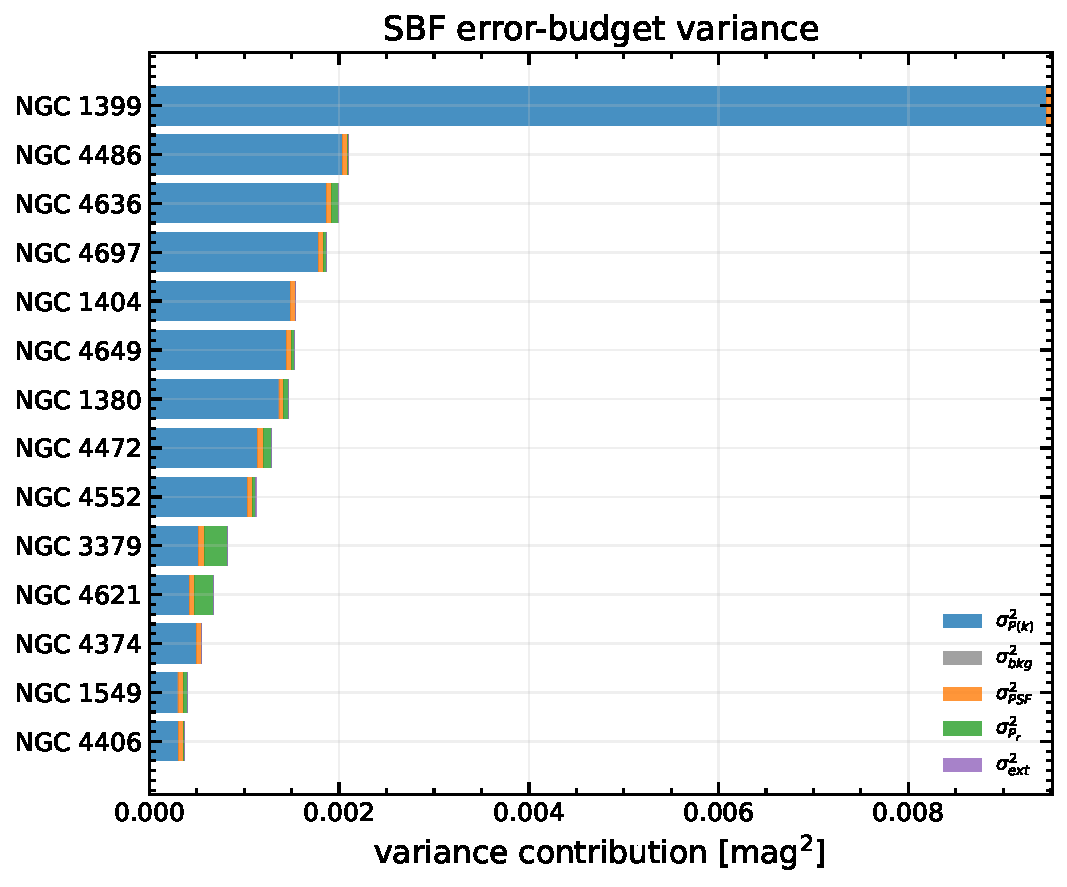
\includegraphics[width=\textwidth]{coursework_error_budget_variance.pdf}
        \end{column}
    \end{columns}
\end{frame}

\begin{frame}{Калибровка $\bar{M}_{150}$}
    \begin{columns}[T,onlytextwidth]
        \begin{column}{0.40\textwidth}
            \small
            \begin{equation*}
                \bar{M}_{150}=\bar{m}_{150}-\mu_{\rm TRGB}
            \end{equation*}
            \begin{equation*}
            \begin{aligned}
                \bar{M}_{150}={}&(-3.454\pm0.013)\\
                &+(1.17\pm0.21)(C-0.40).
            \end{aligned}
            \end{equation*}
            \begin{itemize}
                \item $C=F090W-F150W$;
                \item $0.40$ mag -- центрирование, не физический нуль;
                \item $\sigma_{\rm int}=0.049$ mag;
                \item WRMS линейной модели: $0.059$ mag.
            \end{itemize}
            \vspace{0.05cm}
            {\scriptsize Серая полоса на графике показывает внутренний разброс калибровки, а не ошибку среднего.}
        \end{column}
        \begin{column}{0.57\textwidth}
            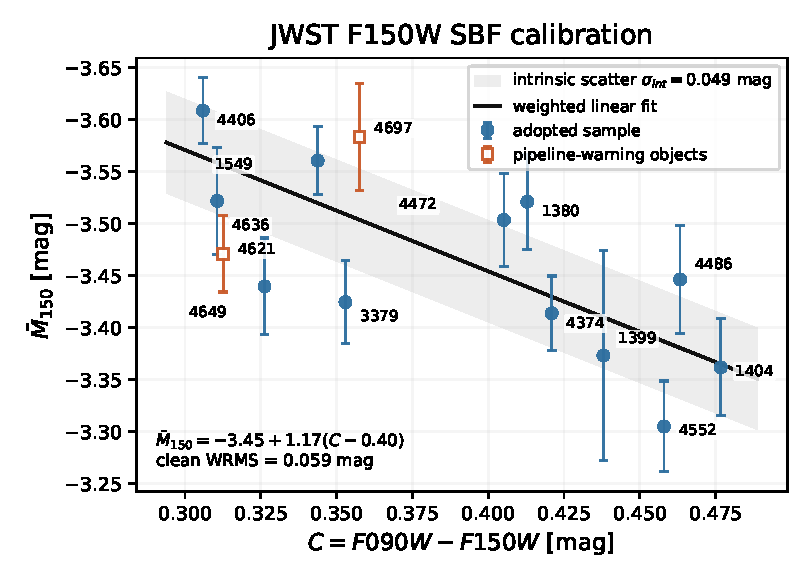
\includegraphics[width=\textwidth]{coursework_Mbar150_color_calibration.pdf}
        \end{column}
    \end{columns}
\end{frame}

\begin{frame}{Почему цвет важен}
    \begin{table}
    \centering
    \begin{tabular}{lcc}
    \toprule
    Модель & WRMS внутри выборки & WRMS leave-one-out \\
    \midrule
    постоянная & 0.091 mag & 0.102 mag \\
    линейная & 0.059 mag & 0.073 mag \\
    квадратичная & 0.059 mag & 0.084 mag \\
    \bottomrule
    \end{tabular}
    \end{table}
    \vspace{0.1cm}
    \begin{itemize}
        \item Постоянная $\bar{M}_{150}$ хуже описывает выборку.
        \item Линейная цветовая калибровка улучшает точность расстояний примерно с $4.7\%$ до $3.4\%$.
        \item Квадратичная модель не даёт устойчивого выигрыша на 12 объектах.
    \end{itemize}
\end{frame}

\begin{frame}{SBF-расстояния против TRGB}
    \begin{columns}[T,onlytextwidth]
        \begin{column}{0.36\textwidth}
            \small
            \begin{itemize}
                \item TRGB -- опорная независимая шкала для всех 14 объектов.
                \item Чистая статистика считается по 12 объектам без warning-флагов.
                \item Среднее смещение: $\Delta_{\rm clean}=0.003\pm0.019$ mag.
                \item WRMS остатков: $0.061$ mag.
                \item В расстояниях: средний сдвиг $0.15\%$, разброс $2.8\%$.
                \item Чёрная линия -- равенство с TRGB, не fit.
                \item Разброс ожидаем: ошибки $\bar{m}_{150}$, TRGB и $\sigma_{\rm int}$.
            \end{itemize}
        \end{column}
        \begin{column}{0.61\textwidth}
            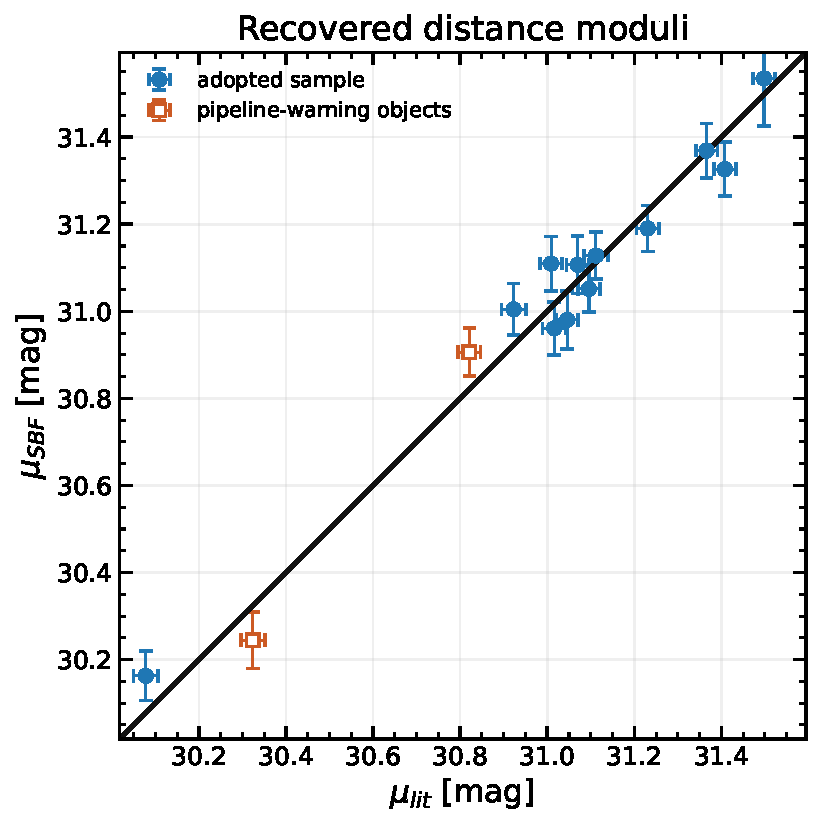
\includegraphics[height=0.74\textheight,width=\textwidth,keepaspectratio]{coursework_mu_sbf_vs_mu_lit.pdf}
        \end{column}
    \end{columns}
\end{frame}

\begin{frame}{Таблица сравнения расстояний (1/2)}
    \tiny
    \setlength{\tabcolsep}{2pt}
    \centering
    \resizebox{\textwidth}{!}{%
    \begin{tabular}{lcccccc}
    \toprule
    Галактика & $\mu_{150}$ & $D_{150}$, Mpc & $\mu_{\rm TRGB}$ & $D_{\rm TRGB}$, Mpc & $\mu_{160,\mathrm{Jensen}}$ & $D_{160,\mathrm{Jensen}}$, Mpc \\
    \midrule
    NGC~1380 & $31.326\pm0.062$ & $18.42\pm0.53$ & $31.408\pm0.025$ & $19.12\pm0.22$ & $31.518\pm0.128$ & $20.12\pm1.19$ \\
    NGC~1399 & $31.535\pm0.109$ & $20.27\pm1.02$ & $31.498\pm0.026$ & $19.93\pm0.24$ & $31.537\pm0.127$ & $20.30\pm1.19$ \\
    NGC~1404 & $31.369\pm0.063$ & $18.78\pm0.54$ & $31.366\pm0.025$ & $18.76\pm0.22$ & $31.488\pm0.134$ & $19.84\pm1.22$ \\
    NGC~1549 & $31.190\pm0.053$ & $17.30\pm0.42$ & $31.231\pm0.026$ & $17.63\pm0.21$ & -- & -- \\
    NGC~3379 & $30.163\pm0.057$ & $10.78\pm0.28$ & $30.078\pm0.028$ & $10.37\pm0.13$ & -- & -- \\
    NGC~4374 & $31.128\pm0.054$ & $16.81\pm0.42$ & $31.112\pm0.027$ & $16.69\pm0.21$ & -- & -- \\
    NGC~4406 & $31.051\pm0.052$ & $16.23\pm0.39$ & $31.096\pm0.025$ & $16.57\pm0.19$ & -- & -- \\
    \bottomrule
    \end{tabular}
    }

    \vspace{0.25cm}
    {\scriptsize
    В таблице показаны модули расстояния и расстояния в Mpc.
    }
\end{frame}

\begin{frame}{Таблица сравнения расстояний (2/2)}
    \tiny
    \setlength{\tabcolsep}{2pt}
    \centering
    \resizebox{\textwidth}{!}{%
    \begin{tabular}{lcccccc}
    \toprule
    Галактика & $\mu_{150}$ & $D_{150}$, Mpc & $\mu_{\rm TRGB}$ & $D_{\rm TRGB}$, Mpc & $\mu_{160,\mathrm{Jensen}}$ & $D_{160,\mathrm{Jensen}}$, Mpc \\
    \midrule
    NGC~4472 & $30.961\pm0.061$ & $15.57\pm0.43$ & $31.016\pm0.027$ & $15.97\pm0.20$ & $31.046\pm0.132$ & $16.19\pm0.98$ \\
    NGC~4486 & $30.980\pm0.067$ & $15.70\pm0.48$ & $31.046\pm0.025$ & $16.19\pm0.19$ & -- & -- \\
    NGC~4552 & $31.005\pm0.059$ & $15.88\pm0.43$ & $30.923\pm0.028$ & $15.30\pm0.20$ & -- & -- \\
    NGC~4621 & $30.906\pm0.055$ & $15.18\pm0.39$ & $30.821\pm0.026$ & $14.59\pm0.17$ & -- & -- \\
    NGC~4636 & $31.107\pm0.066$ & $16.65\pm0.51$ & $31.070\pm0.026$ & $16.37\pm0.20$ & -- & -- \\
    NGC~4649 & $31.110\pm0.063$ & $16.67\pm0.48$ & $31.009\pm0.025$ & $15.91\pm0.18$ & $31.001\pm0.135$ & $15.86\pm0.98$ \\
    NGC~4697 & $30.245\pm0.065$ & $11.19\pm0.34$ & $30.324\pm0.028$ & $11.61\pm0.15$ & -- & -- \\
    \bottomrule
    \end{tabular}
    }

    \vspace{0.25cm}
    {\scriptsize
    Прочерк означает отсутствие соответствующего F160W-измерения в пересечении с Jensen et al. 2015.
    NGC~4621 и NGC~4697 показаны для полноты, но не входят в clean-статистику.
    }
\end{frame}

\begin{frame}{Проверка leave-one-out}
    \begin{columns}[T]
        \begin{column}{0.43\textwidth}
            \begin{itemize}
                \item Для каждой галактики калибровка строится без неё.
                \item Затем расстояние восстанавливается как для новой галактики.
                \item WRMS остатков: $0.073$ mag.
                \item Это соответствует примерно $3.4\%$ по расстоянию.
            \end{itemize}
            \begin{equation*}
                \frac{\Delta D}{D}\simeq\frac{\ln 10}{5}\Delta\mu\simeq0.46\Delta\mu
            \end{equation*}
        \end{column}
        \begin{column}{0.54\textwidth}
            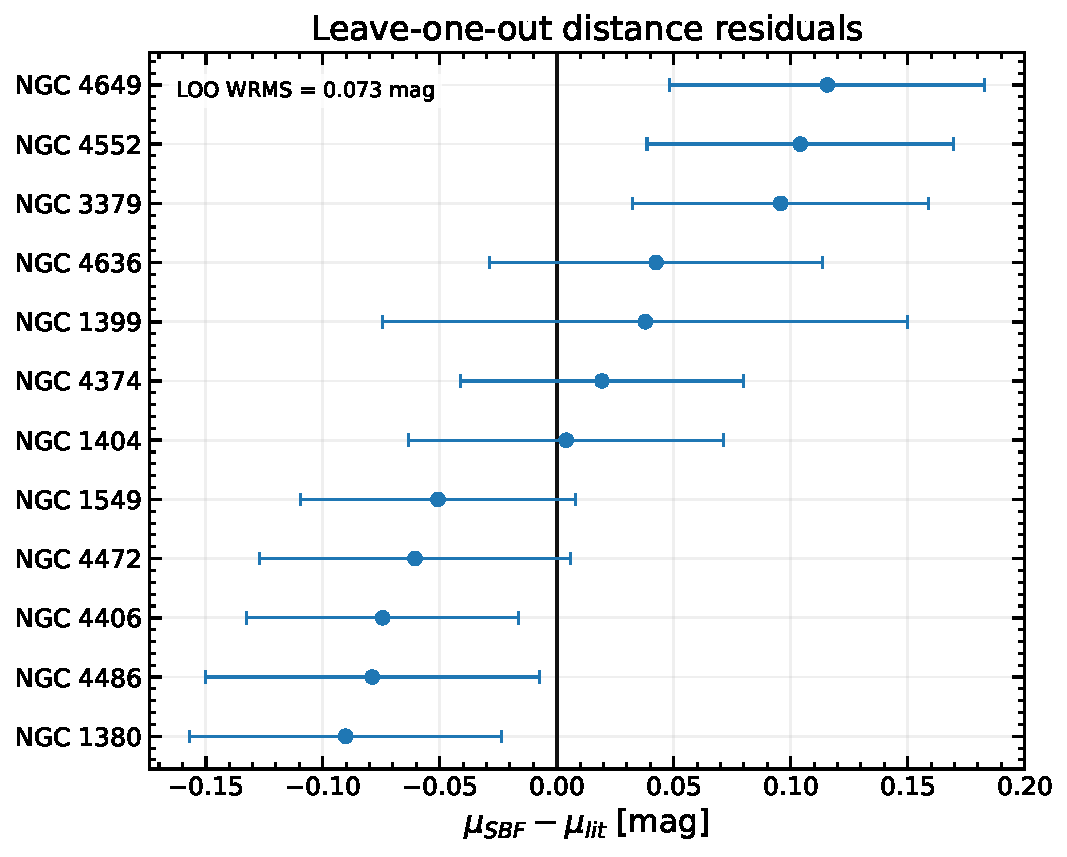
\includegraphics[width=\textwidth]{coursework_leave_one_out_residuals.pdf}
        \end{column}
    \end{columns}
\end{frame}

\begin{frame}{Сравнение с Jensen et al. 2015}
    \begin{columns}[T,onlytextwidth]
        \begin{column}{0.34\textwidth}
            \small
            \begin{itemize}
                \item Сравниваются две SBF-реализации:
                JWST/F150W и HST/F160W.
                \item Общих галактик: 5.
                \item Среднее смещение: $\Delta=-0.063\pm0.067$ mag.
                \item WRMS остатков: $0.105$ mag.
                \item В расстояниях: $-2.9\%$.
            \end{itemize}
        \end{column}
        \begin{column}{0.63\textwidth}
            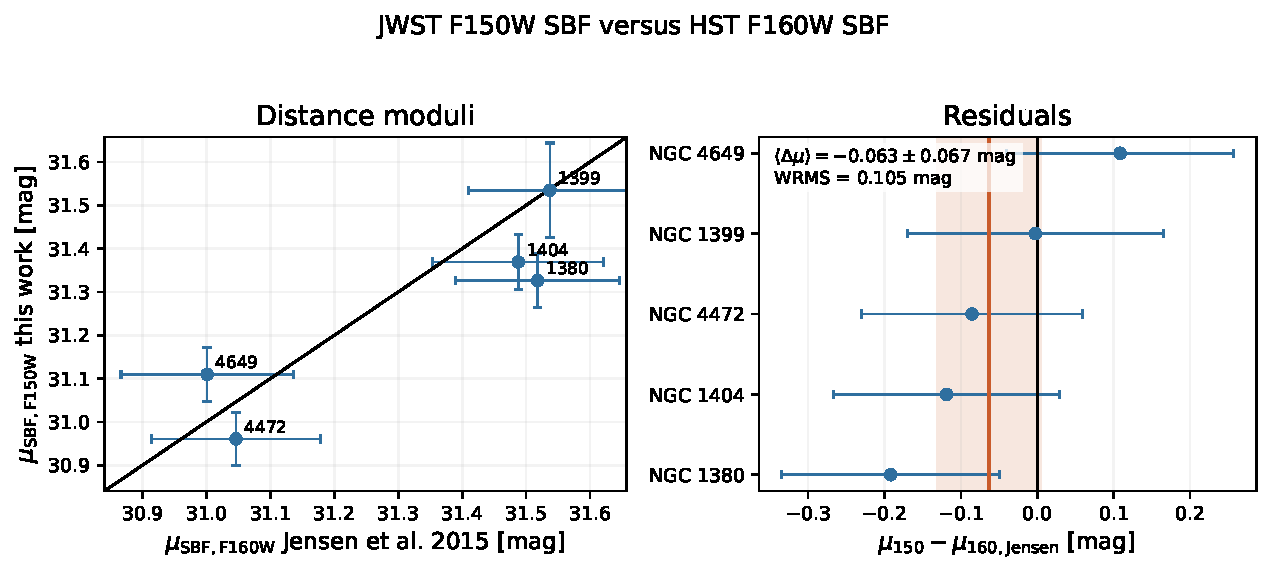
\includegraphics[width=\textwidth]{coursework_jensen_f160w_comparison.pdf}
        \end{column}
    \end{columns}
\end{frame}

\begin{frame}{Пять общих галактик с Jensen et al. 2015}
    \centering
    \scriptsize
    \setlength{\tabcolsep}{3pt}
    \resizebox{\textwidth}{!}{%
    \begin{tabular}{lcccccc}
    \toprule
    Галактика & $\mu_{150}$ & $D_{150}$, Mpc & $\mu_{160,\rm Jensen}$ & $D_{160,\rm Jensen}$, Mpc & $\Delta\mu$ & $D_{150}/D_{160}$ \\
    \midrule
    NGC~1380 & 31.326 & $18.42\pm0.53$ & 31.518 & $20.12\pm1.19$ & $-0.192$ & 0.915 \\
    NGC~1399 & 31.535 & $20.27\pm1.02$ & 31.537 & $20.30\pm1.19$ & $-0.003$ & 0.999 \\
    NGC~1404 & 31.369 & $18.78\pm0.54$ & 31.488 & $19.84\pm1.22$ & $-0.119$ & 0.947 \\
    NGC~4472 & 30.961 & $15.57\pm0.43$ & 31.046 & $16.19\pm0.98$ & $-0.085$ & 0.961 \\
    NGC~4649 & 31.110 & $16.67\pm0.48$ & 31.001 & $15.86\pm0.98$ & $+0.109$ & 1.051 \\
    \bottomrule
    \end{tabular}
    }

    \vspace{0.35cm}
    \begin{block}{Интерпретация таблицы}
        Четыре из пяти объектов дают меньшие F150W/TRGB-расстояния, чем восстановленная шкала Jensen/F160W. Среднее смещение мало относительно объединённых ошибок и имеет ожидаемый знак для перехода от старой Cepheid/optical-SBF шкалы к TRGB-основанной шкале Virgo/Fornax.
    \end{block}
\end{frame}

\begin{frame}{Как интерпретировать расхождения}
    \begin{itemize}
        \item С TRGB: средний сдвиг практически нулевой, WRMS $0.061$ mag.
        \item С Jensen/F160W: наши расстояния немного короче, $-0.063\pm0.067$ mag.
        \item Это согласуется с тем, что TRGB-основанная шкала Virgo/Fornax короче старой Cepheid/optical-SBF шкалы на $3$--$4\%$.
        \item NGC 1380: $\Delta\mu_{150-\rm TRGB}=-0.082$ mag, но это всего около $1.2\sigma$.
        \item NGC 1399: формально пайплайн прошёл, но ошибка $\bar{m}_{150}$ велика: $0.098$ mag; объект имеет малый вес.
    \end{itemize}
\end{frame}

% \begin{frame}{Объекты с предупреждениями}
%     \begin{columns}[T,onlytextwidth]
%         \begin{column}{0.48\textwidth}
%             \begin{block}{NGC 4621 и NGC 4697}
%                 Они оставлены в полной таблице, но исключены из clean-статистики: у NGC~4621 есть предупреждение по Sersic-модели, у NGC~4697 -- сбой real-only изофотной ветки и предупреждение по Sersic-модели.
%             \end{block}
%             \begin{block}{NGC 1399}
%                 Формально чистый, но имеет большую ошибку $\bar{m}_{150}=28.125\pm0.098$ mag. Взвешенная калибровка автоматически даёт ей малый вес.
%             \end{block}
%         \end{column}
%         \begin{column}{0.48\textwidth}
%             \begin{block}{NGC 1380}
%                 Самая заметная отрицательная TRGB-разность: $\Delta\mu=-0.082\pm0.067$ mag, около $1.2\sigma$. Это диагностический объект, но не основание выкидывать точку.
%             \end{block}
%             \begin{block}{Тактика}
%                 В докладе важно не прятать эти точки: они показывают реальный уровень индивидуальной систематики, а не ломают среднюю калибровку.
%             \end{block}
%         \end{column}
%     \end{columns}
% \end{frame}

\begin{frame}{Диагностика систематик}
    \begin{columns}[T,onlytextwidth]
        \begin{column}{0.28\textwidth}
            \small
            \begin{itemize}
                \item Проверены остатки против цвета, расстояния, $\sigma_{P(k)}$, PSF и $P_r/P_0$.
                \item На 12 объектах это не строгая статистика.
                \item Цель -- увидеть явный провал пайплайна.
                \item Очевидного одного доминирующего тренда нет.
            \end{itemize}
        \end{column}
        \begin{column}{0.69\textwidth}
            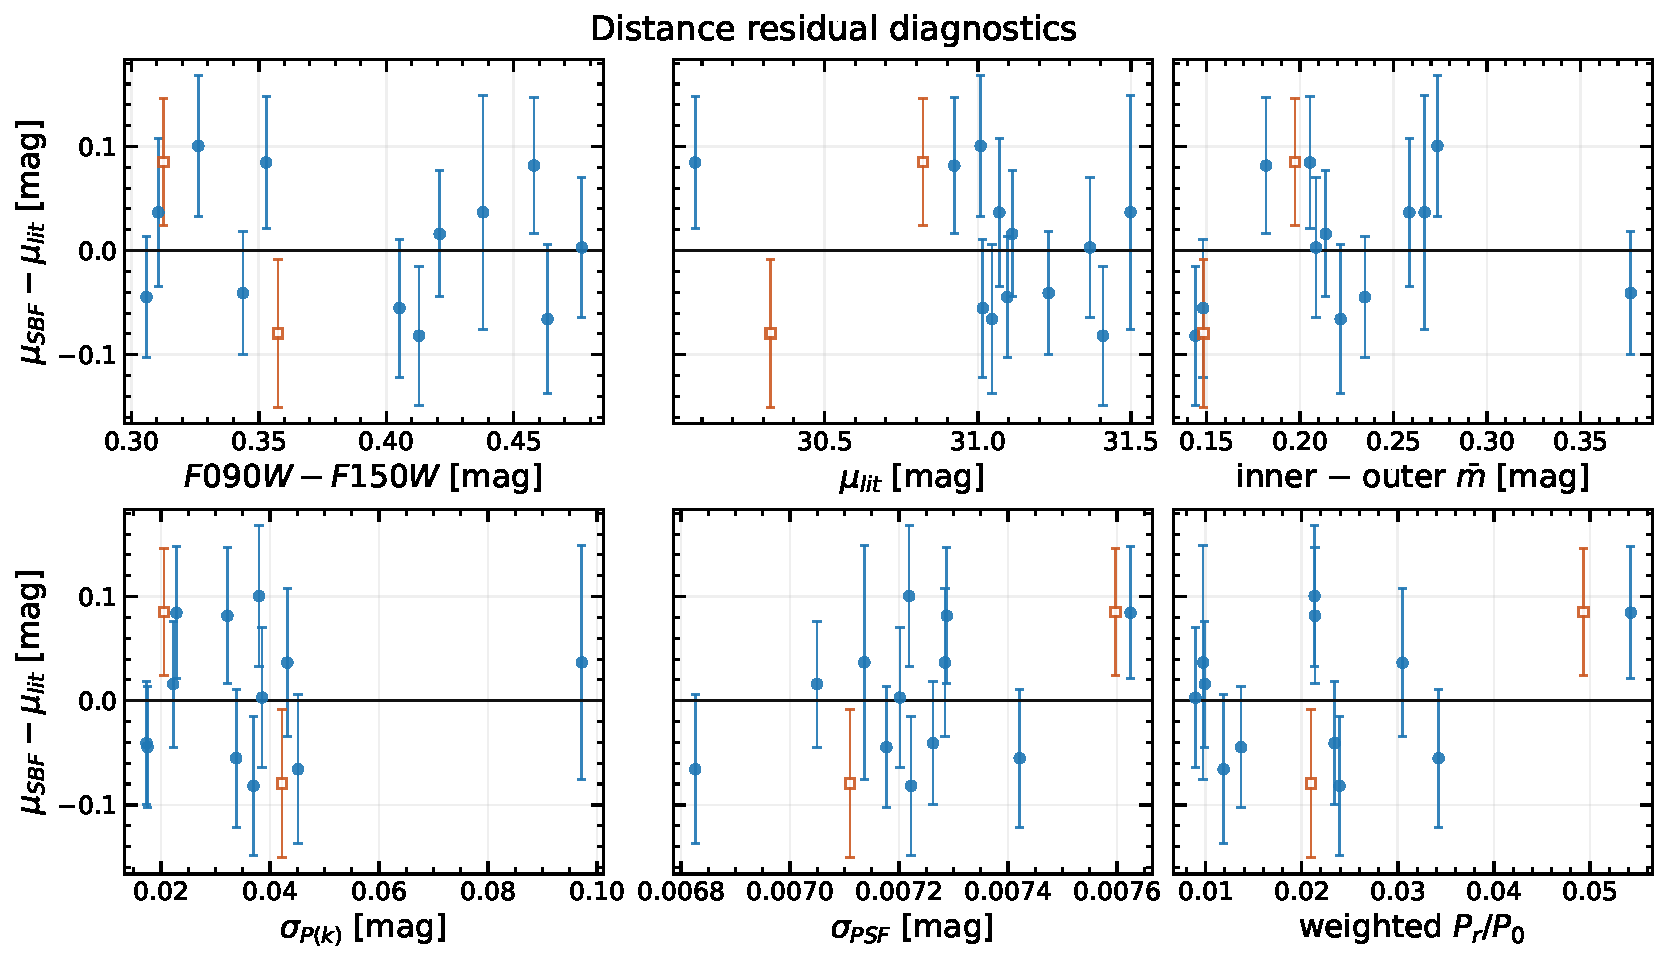
\includegraphics[width=\textwidth]{coursework_residual_diagnostics_grid.pdf}
        \end{column}
    \end{columns}
\end{frame}

\begin{frame}{Итоги}
    \begin{itemize}
        \item Измерены $\bar{m}_{150}$ для 14 галактик JWST GO-3055.
        \item Получена F150W SBF-калибровка по TRGB-шкале:
        \begin{equation*}
            \bar{M}_{150}=(-3.454\pm0.013)+(1.17\pm0.21)(C-0.40).
        \end{equation*}
        \item Цвет уменьшает leave-one-out разброс с $0.102$ до $0.073$ mag.
        \item Относительно TRGB среднее смещение равно $0.003\pm0.019$ mag.
        \item Относительно Jensen/F160W найдено смещение $-0.063\pm0.067$ mag, согласованное по знаку и величине с известным отличием шкал.
    \end{itemize}
\end{frame}

\begin{frame}
    \centering
    \vspace{1.5cm}
    {\Huge Спасибо за внимание}
\end{frame}

\end{document}
